\documentclass[a4paper,oneside,11pt]{book}

% Package yang diperlukan
\usepackage{graphicx}
\usepackage{titling}
\usepackage{geometry}
\usepackage{listings}
\usepackage{xcolor}
\usepackage{float}
\usepackage{hyperref}
\usepackage{indentfirst}
\usepackage{longtable}
\usepackage{array}

% Pengaturan margin
\geometry{
    left=3cm,
    right=2.5cm,
    top=3cm,
    bottom=3cm
}
% Pengaturan untuk kode HTML
\definecolor{codegreen}{rgb}{0,0.6,0}
\definecolor{codegray}{rgb}{0.5,0.5,0.5}
\definecolor{codepurple}{rgb}{0.58,0,0.82}
\definecolor{backcolour}{rgb}{0.95,0.95,0.92}

\lstdefinestyle{javastyle}{
    language=Java,
    backgroundcolor=\color{backcolour},
    commentstyle=\color{codegreen},
    keywordstyle=\color{blue}\bfseries,
    numberstyle=\tiny\color{codegray},
    stringstyle=\color{orange},
    basicstyle=\ttfamily\footnotesize,
    breakatwhitespace=false,
    breaklines=true,
    captionpos=b,
    keepspaces=true,
    numbers=left,
    numbersep=5pt,
    showspaces=false,
    showstringspaces=false,
    showtabs=false,
    tabsize=2,
    frame=single
}


\title{Laporan Praktikum \\ Praktikum Pengujian Perangkat Lunak\\
Pertemuan 2\\
 Life Cycle}
\author{Nama Mahasiswa: Januarsyah Akbar (24/535846/SV/24314)}
\date{\today}

\begin{document}

% Halaman judul
\begin{titlingpage}
\begin{center}
\vspace{4cm}
\begin{huge} 
\textbf{\thetitle} \\
\end{huge}
\vspace{2cm}

\includegraphics[height=8cm]{lambang ugm.png}\\
\begin{Large}
\vspace{4cm}
\theauthor\\
Kelas B2 \\
\end{Large}
\begin{large}
Dosen Pengampu: Divi Galih Prasetyo Putri, S.Kom., M.Kom., Ph.D.\\
\end{large}
\vspace{2cm}
\thedate
\end{center}
\end{titlingpage}

% Daftar Isi
\tableofcontents
\newpage
\chapter{Tujuan Praktikum}
\begin{enumerate}
    \item Mahasiswa memahami life cycle dan anotasi yang ada pada JUnit
    \item Mahasiswa mampu mengimplementasikan anotasi pada pengujian unit
\end{enumerate}
\chapter{Langkah Praktikum}
\section*{Resources}
Download source code praktikum pada link berikut: \\
\url{https://github.com/januarsyah901/PPPL/tree/main/Pertemuan%202}
\section{Unit Test: WalletTest.java}

\subsection{BeforeAll}
Metode \texttt{setUp()} yang dianotasi dengan \texttt{@BeforeAll} dijalankan sekali sebelum semua test method dalam class dijalankan. Metode ini bersifat statis dan digunakan untuk inisialisasi resource yang didapatkan bersama oleh semua test.

\begin{lstlisting}[style=javastyle]
@BeforeAll
static void setUp() {
    staticSharedWallet = new Wallet();
    staticSharedWallet.setOwner("Shared Wallet for All Tests");
    staticSharedWallet.addMoney(500_000);
    staticSharedWallet.addCard("MANDIRI Debit");
    staticSharedWallet.addCard("BCA Visa");
}
\end{lstlisting}

Pada contoh ini, method \texttt{setUp()} membuat sebuah instance \texttt{Wallet} statis yang dibagikan untuk semua test. Wallet ini diinisialisasi dengan nama pemilik, saldo awal 500.000, dan dua kartu kredit.

\subsection{BeforeEach}
Metode \texttt{setUpEachTest()} yang dianotasi dengan \texttt{@BeforeEach} dijalankan sebelum setiap test method dijalankan. Metode ini digunakan untuk menginisialisasi resource yang diperlukan oleh setiap test secara individual.

\begin{lstlisting}[style=javastyle]
@BeforeEach
void setUpEachTest() {
    wallet = new Wallet();
    wallet.setOwner("Kadal Coklat");
    wallet.addMoney(100_000);
    wallet.addCard("BRI BritAma");
}
\end{lstlisting}

Untuk setiap test, dibuat instance Wallet baru dengan pemilik "Kadal Coklat", saldo awal 100.000, dan satu kartu debit. Ini memastikan setiap test memiliki state yang fresh dan tidak terpengaruh oleh test sebelumnya.

\subsection{AfterAll}
Metode \texttt{cleanUp()} yang dianotasi dengan \texttt{@AfterAll} dijalankan sekali setelah semua test method selesai dijalankan. Metode ini digunakan untuk membersihkan resource global.

\begin{lstlisting}[style=javastyle]
@AfterAll
static void cleanUp() {
    staticSharedWallet = null;
}
\end{lstlisting}

Method ini membebaskan reference ke \texttt{staticSharedWallet} dengan mengatur nilainya menjadi null, memastikan resource global dibersihkan setelah semua test selesai.

\subsection{AfterEach}
Metode \texttt{tearDownEachTest()} yang dianotasi dengan \texttt{@AfterEach} dijalankan setelah setiap test method selesai dijalankan. Metode ini digunakan untuk membersihkan resource lokal.

\begin{lstlisting}[style=javastyle]
@AfterEach
void tearDownEachTest() {
    wallet = null;
}
\end{lstlisting}

Setelah setiap test selesai, object \texttt{wallet} yang telah digunakan dibebaskan dengan mengatur nilainya menjadi null. Ini mencegah memory leak dan memastikan state bersih untuk test berikutnya.

\subsection{Test}
Bagian ini berisi lima test method yang masing-masing menguji fungsionalitas berbeda dari class Wallet.

\subsubsection{Order Annotation}
Untuk mengontrol urutan eksekusi test method, digunakan anotasi \texttt{@Order} bersama dengan \texttt{@TestMethodOrder}. Pada class level, ditambahkan:

\begin{lstlisting}[style=javastyle]
@TestMethodOrder(MethodOrderer.OrderAnnotation.class)
class WalletTest {
    ...
}
\end{lstlisting}

Kemudian, setiap test method dianotasi dengan \texttt{@Order(n)} untuk menentukan urutan eksekusinya:

\begin{lstlisting}[style=javastyle]
@Test
@Order(1)
void testAddAndTakeMoney() { ... }

@Test
@Order(2)
void testAddAndTakeCard() { ... }
\end{lstlisting}

Anotasi \texttt{@TestMethodOrder(MethodOrderer.OrderAnnotation.class)} memberi tahu JUnit untuk menjalankan test method sesuai dengan urutan angka yang ditetapkan pada anotasi \texttt{@Order}. Nilai yang lebih kecil dijalankan terlebih dahulu. Ini berguna ketika test-test memiliki ketergantungan atau ketika perlu memastikan test dijalankan dalam urutan tertentu.

\subsubsection{testAddAndTakeMoney()}
Test method ini menguji fungsionalitas penambahan dan pengambilan uang dari wallet.

\begin{lstlisting}[style=javastyle]
@Test
@Order(1)
void testAddAndTakeMoney() {
    assertEquals(100_000, wallet.getTotalMoney());
    wallet.addMoney(50_000);
    assertEquals(150_000, wallet.getTotalMoney());
    boolean success = wallet.takeMoney(70_000);
    assertTrue(success);
    assertEquals(80_000, wallet.getTotalMoney());
    success = wallet.takeMoney(100_000);
    assertFalse(success);
    assertEquals(80_000, wallet.getTotalMoney());
}
\end{lstlisting}

Test ini memverifikasi bahwa saldo awal wallet adalah 100.000. Kemudian, penambahan 50.000 menghasilkan saldo 150.000 sebagaimana diharapkan. Selanjutnya, pengambilan 70.000 berhasil dilakukan dan saldo menjadi 80.000. Terakhir, pengambilan 100.000 gagal dilakukan karena saldo tidak mencukupi, dan saldo tetap berada di 80.000.

\subsubsection{testAddAndTakeCard()}
Test method ini menguji fungsi penambahan dan pengambilan kartu dari wallet.

\begin{lstlisting}[style=javastyle]
@Test
@Order(2)
void testAddAndTakeCard() {
    assertEquals(1, wallet.getCards().size());
    wallet.addCard("BNI Taplus");
    wallet.addCard("OVO");
    assertEquals(3, wallet.getCards().size());
    assertTrue(wallet.getCards().contains("BNI Taplus"));
    String taken = wallet.takeCard("OVO");
    assertEquals("OVO", taken);
    assertFalse(wallet.getCards().contains("OVO"));
    assertEquals(2, wallet.getCards().size());
}
\end{lstlisting}

Test ini memverifikasi bahwa wallet awalnya memiliki 1 kartu. Setelah penambahan 2 kartu baru ("BNI Taplus" dan "OVO"), jumlah total kartu menjadi 3. Kemudian, test memastikan bahwa kartu yang baru ditambahkan berhasil ditemukan dalam wallet. Terakhir, pengambilan kartu "OVO" berhasil dilakukan, menghapusnya dari wallet sehingga sisa kartu kembali menjadi 2.
\newpage
\subsubsection{testTakeNonExistentCard()}
Test method ini menguji pengambilan kartu yang tidak ada di wallet.

\begin{lstlisting}[style=javastyle]
@Test
@Order(3)
void testTakeNonExistentCard() {
    String result = wallet.takeCard("Gopay");
    assertNull(result);
    assertEquals(1, wallet.getCards().size());
}
\end{lstlisting}

Test ini memverifikasi bahwa ketika mencoba mengambil kartu yang tidak ada ("Gopay"), method mengembalikan null dan jumlah kartu tidak berubah.

\subsubsection{testOwner()}
Test method ini menguji fungsionalitas get dan set pemilik wallet.

\begin{lstlisting}[style=javastyle]
@Test
@Order(4)
void testOwner() {
    assertEquals("Kadal Coklat", wallet.getOwner());
    wallet.setOwner("Janu Si Kadal");
    assertEquals("Janu Si Kadal", wallet.getOwner());
}
\end{lstlisting}

Test ini memverifikasi pemilik awal sesuai dengan yang ditetapkan di BeforeEach, dan pengubahan pemilik berhasil disimpan dan dapat diambil kembali.
\subsubsection{testStaticWalletStillExists()}
Test method ini menguji bahwa wallet statis yang dibuat di BeforeAll masih ada dan tetap mempertahankan nilainya.

\begin{lstlisting}[style=javastyle]
@Test
@Order(5)
void testStaticWalletStillExists() {
    assertNotNull(staticSharedWallet);
    assertEquals("Shared Wallet for All Tests", staticSharedWallet.getOwner());
    assertEquals(500_000, staticSharedWallet.getTotalMoney());
    assertEquals(2, staticSharedWallet.getCards().size());
}
\end{lstlisting}

Test ini memverifikasi bahwa wallet statis yang dibagi tidak null dan tetap mempertahankan nilai yang ditetapkan di BeforeAll, menunjukkan bahwa resource global tidak terpengaruh oleh test-test individual.

\subsubsection{Test Passed}
\begin{figure}[H]
    \centering
    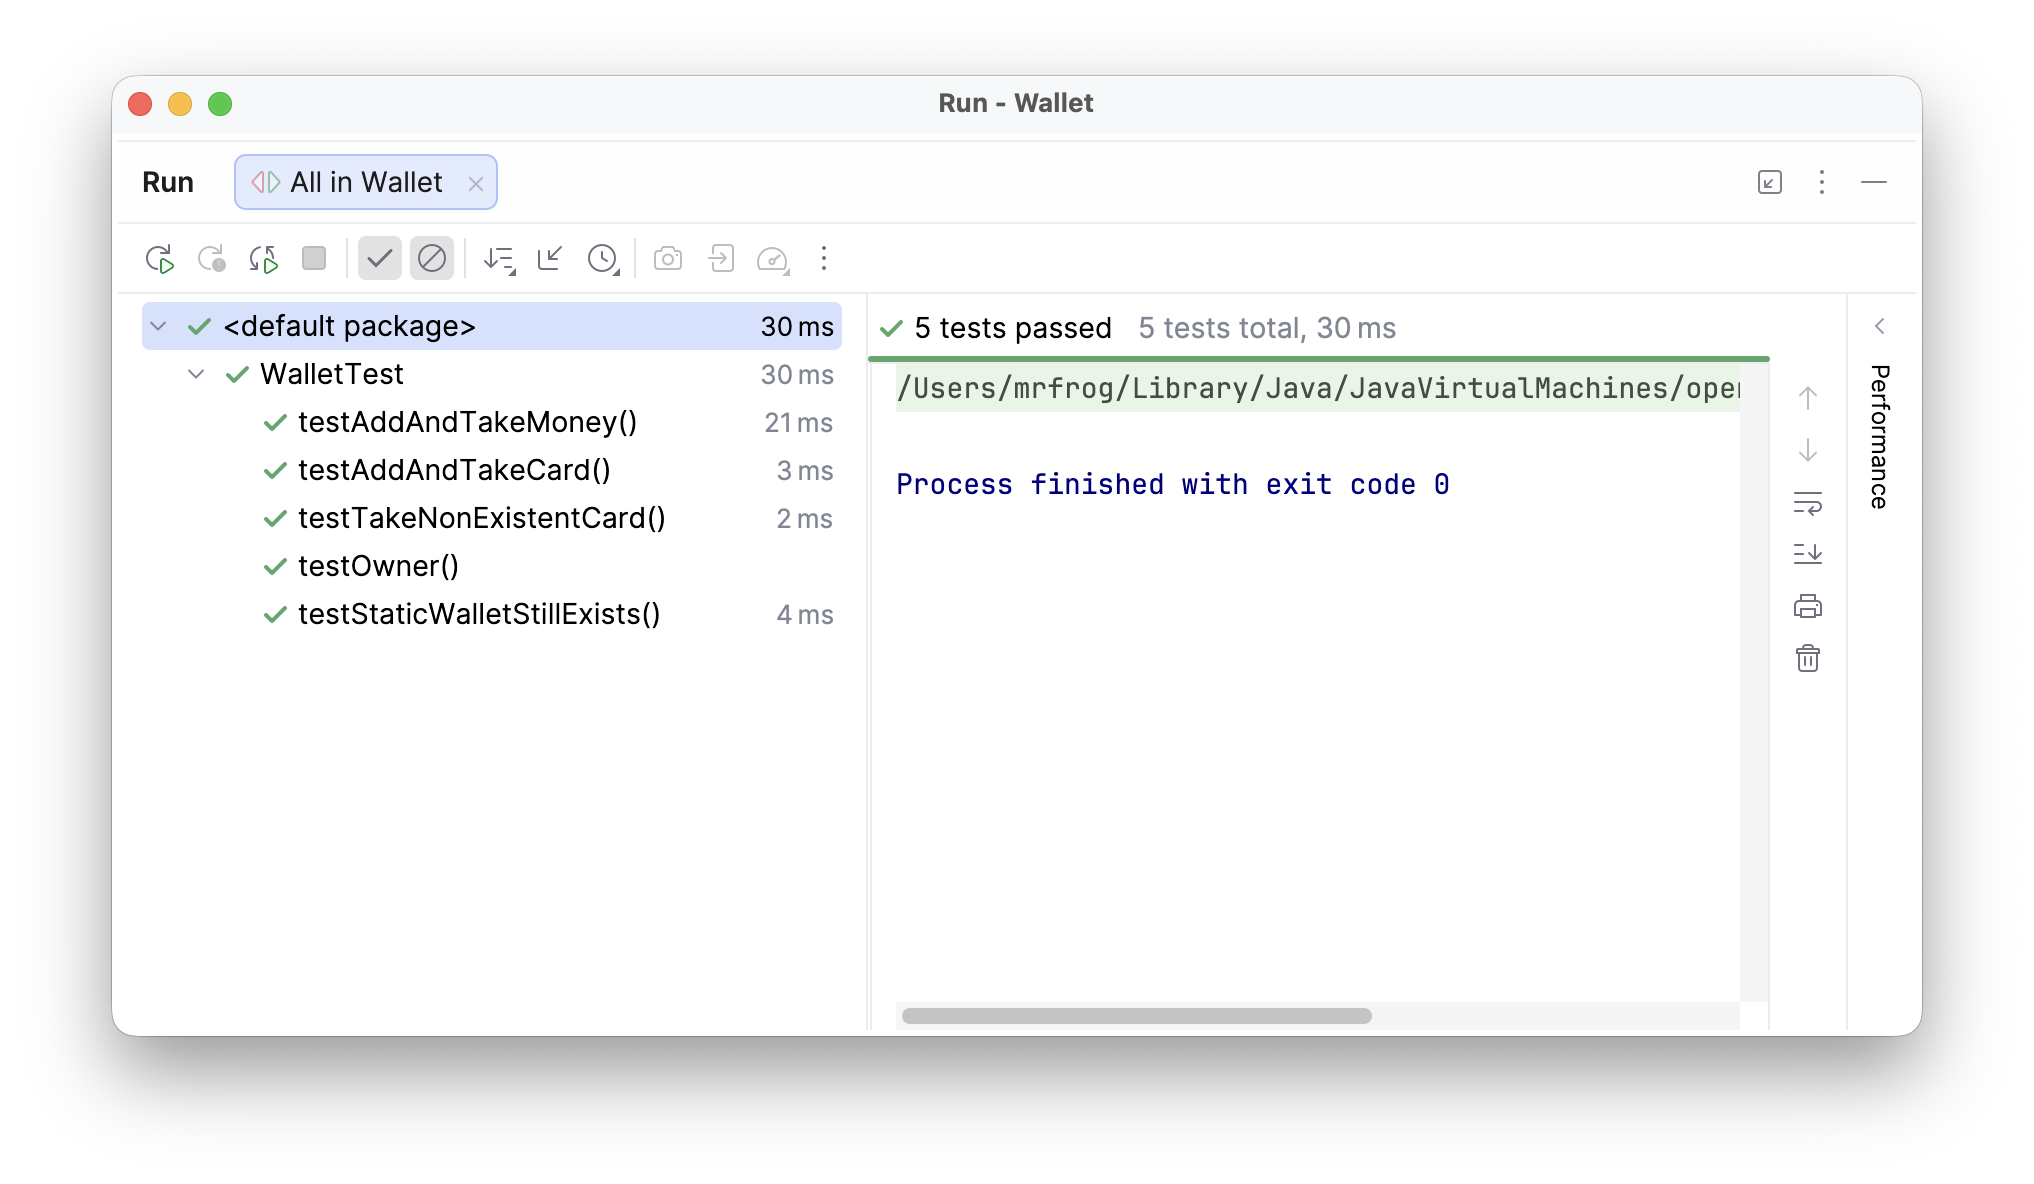
\includegraphics[width=0.5\textwidth]{test passed.png}
    \caption{Hasil test yang berhasil}
\end{figure}
\chapter{Kesimpulan}
Pada praktikum ini, saya belajar tentang anotasi yang ada pada JUnit, seperti BeforeAll, BeforeEach, AfterAll, AfterEach, dan Test. Anotasi BeforeAll digunakan untuk mengeksekusi kode sebelum semua pengujian dijalankan, sedangkan BeforeEach digunakan untuk mengeksekusi kode sebelum setiap pengujian dijalankan. Anotasi AfterAll digunakan untuk mengeksekusi kode setelah semua pengujian selesai dijalankan, sedangkan AfterEach digunakan untuk mengeksekusi kode setelah setiap pengujian selesai dijalankan.
\end{document}  